% VisionAssist Senior Design Poster
% Iowa State University SDDEC25-01
% A0 Portrait Format Poster

\documentclass[25pt, a0paper, portrait]{tikzposter}

% Essential packages
\usepackage[utf8]{inputenc}
\usepackage[T1]{fontenc}
\usepackage{lmodern}
\usepackage{graphicx}
\usepackage{amsmath}
\usepackage{amssymb}
\usepackage{microtype}
\usepackage{booktabs}

% TikZ libraries for coordinate calculations
\usetikzlibrary{calc}

% Bibliography setup - using relative path to main project references
\usepackage[backend=biber, style=ieee, sorting=none]{biblatex}
\addbibresource{../references.bib}

% Load poster theme configuration
\makeatletter
% Poster Configuration: ISU Theme Colors and Styling
% For VisionAssist Senior Design Project

% ===== COLOR DEFINITIONS =====

% Iowa State University Brand Colors
\definecolor{isucardinal}{RGB}{200, 16, 46}    % ISU Cardinal Red (#C8102E)
\definecolor{isugold}{RGB}{241, 190, 72}       % ISU Gold (#F1BE48)

% Supporting grayscale colors for readability
\definecolor{darkgray}{RGB}{60, 60, 60}        % Dark text color
\definecolor{lightgray}{RGB}{240, 240, 240}    % Light background
\definecolor{white}{RGB}{255, 255, 255}        % Pure white

% ===== TIKZPOSTER COLOR STYLE =====

% Define custom color palette for tikzposter
\definecolorstyle{ISUStyle}{
  % Fill colors
  \colorlet{colorOne}{isucardinal}
  \colorlet{colorTwo}{isugold}
  \colorlet{colorThree}{lightgray}
}{
  % Derived colors for various poster elements
  \colorlet{backgroundcolor}{white}
  \colorlet{framecolor}{isucardinal}
  \colorlet{titlefgcolor}{white}
  \colorlet{titlebgcolor}{isucardinal}
  \colorlet{blocktitlebgcolor}{isucardinal}
  \colorlet{blocktitlefgcolor}{white}
  \colorlet{blockbodybgcolor}{white}
  \colorlet{blockbodyfgcolor}{darkgray}
  \colorlet{innerblocktitlebgcolor}{isugold}
  \colorlet{innerblocktitlefgcolor}{darkgray}
  \colorlet{innerblockbodybgcolor}{lightgray}
  \colorlet{innerblockbodyfgcolor}{darkgray}
  \colorlet{notefgcolor}{darkgray}
  \colorlet{notebgcolor}{isugold!50}
}

% ===== BACKGROUND STYLE =====

\definebackgroundstyle{ISUBackground}{
  \draw[line width=0pt, color=white, fill=white]
  (bottomleft) rectangle (topright);
}

% ===== BLOCK STYLING =====

% Custom block style with rounded corners and cardinal border
\defineblockstyle{ISUBlock}{
  titlewidthscale=1.0, bodywidthscale=1.0, titleleft,
  titleoffsetx=0pt, titleoffsety=0pt, bodyoffsetx=0pt, bodyoffsety=0pt,
  bodyverticalshift=15pt, roundedcorners=15, linewidth=5pt,  % Added vertical shift for spacing
  titleinnersep=18pt, bodyinnersep=25pt  % Increased padding for better whitespace
}{
  \draw[color=framecolor, fill=blocktitlebgcolor,
  rounded corners=\blockroundedcorners, line width=\blocklinewidth]
  (blocktitle.south west) rectangle (blocktitle.north east);
  \draw[color=framecolor, fill=blockbodybgcolor,
  rounded corners=\blockroundedcorners, line width=\blocklinewidth]
  (blockbody.south west) rectangle (blockbody.north east);
}

% Inner block style for nested content
\defineinnerblockstyle{ISUInnerBlock}{
  titlewidthscale=1.0, bodywidthscale=1.0, titleleft,
  titleoffsetx=0pt, titleoffsety=0pt, bodyoffsetx=0pt, bodyoffsety=0pt,
  bodyverticalshift=0pt, roundedcorners=10, linewidth=3pt,
  titleinnersep=10pt, bodyinnersep=15pt
}{
  \draw[color=framecolor, fill=innerblocktitlebgcolor,
  rounded corners=\innerblockroundedcorners]
  (innerblocktitle.south west) rectangle (innerblocktitle.north east);
  \draw[color=framecolor, fill=innerblockbodybgcolor,
  rounded corners=\innerblockroundedcorners]
  (innerblockbody.south west) rectangle (innerblockbody.north east);
}

% ===== TITLE STYLE =====

\definetitlestyle{ISUTitle}{
  width=\paperwidth, roundedcorners=0, linewidth=5pt, innersep=20pt,
  titletotopverticalspace=0mm, titletoblockverticalspace=40mm  % More space after title
}{
  \draw[color=framecolor, fill=titlebgcolor, line width=\titlelinewidth]
  (\titleposleft,\titleposbottom) rectangle (\titleposright,\titlepostop);
}

% ===== FONT CONFIGURATION =====

% Use sans-serif fonts for better readability at distance
\renewcommand{\familydefault}{\sfdefault}

% Adjust spacing for large format
\setlength{\parskip}{1.5em}  % Increased paragraph spacing for readability
\setlength{\columnsep}{5cm}  % More whitespace between columns

% ===== APPLY STYLES =====

\usecolorstyle{ISUStyle}
\usebackgroundstyle{ISUBackground}
\useblockstyle{ISUBlock}
\useinnerblockstyle{ISUInnerBlock}
\usetitlestyle{ISUTitle}

% ===== TIKZPOSTER OPTIONS =====

% Additional configuration for better layout
\tikzposterlatexaffectionproofoff{}
% Remove tikzposter watermark

\makeatother

% Document metadata
\title{\parbox{\linewidth}{\centering VisionAssist:\\Real-Time AI Eye
Tracking for Medical Assistive Technology}}
\author{Iowa State University Senior Design Team SDDEC25--01}
\institute{Department of Electrical and Computer Engineering}

% Set title graphic (ISU logo)
\titlegraphic{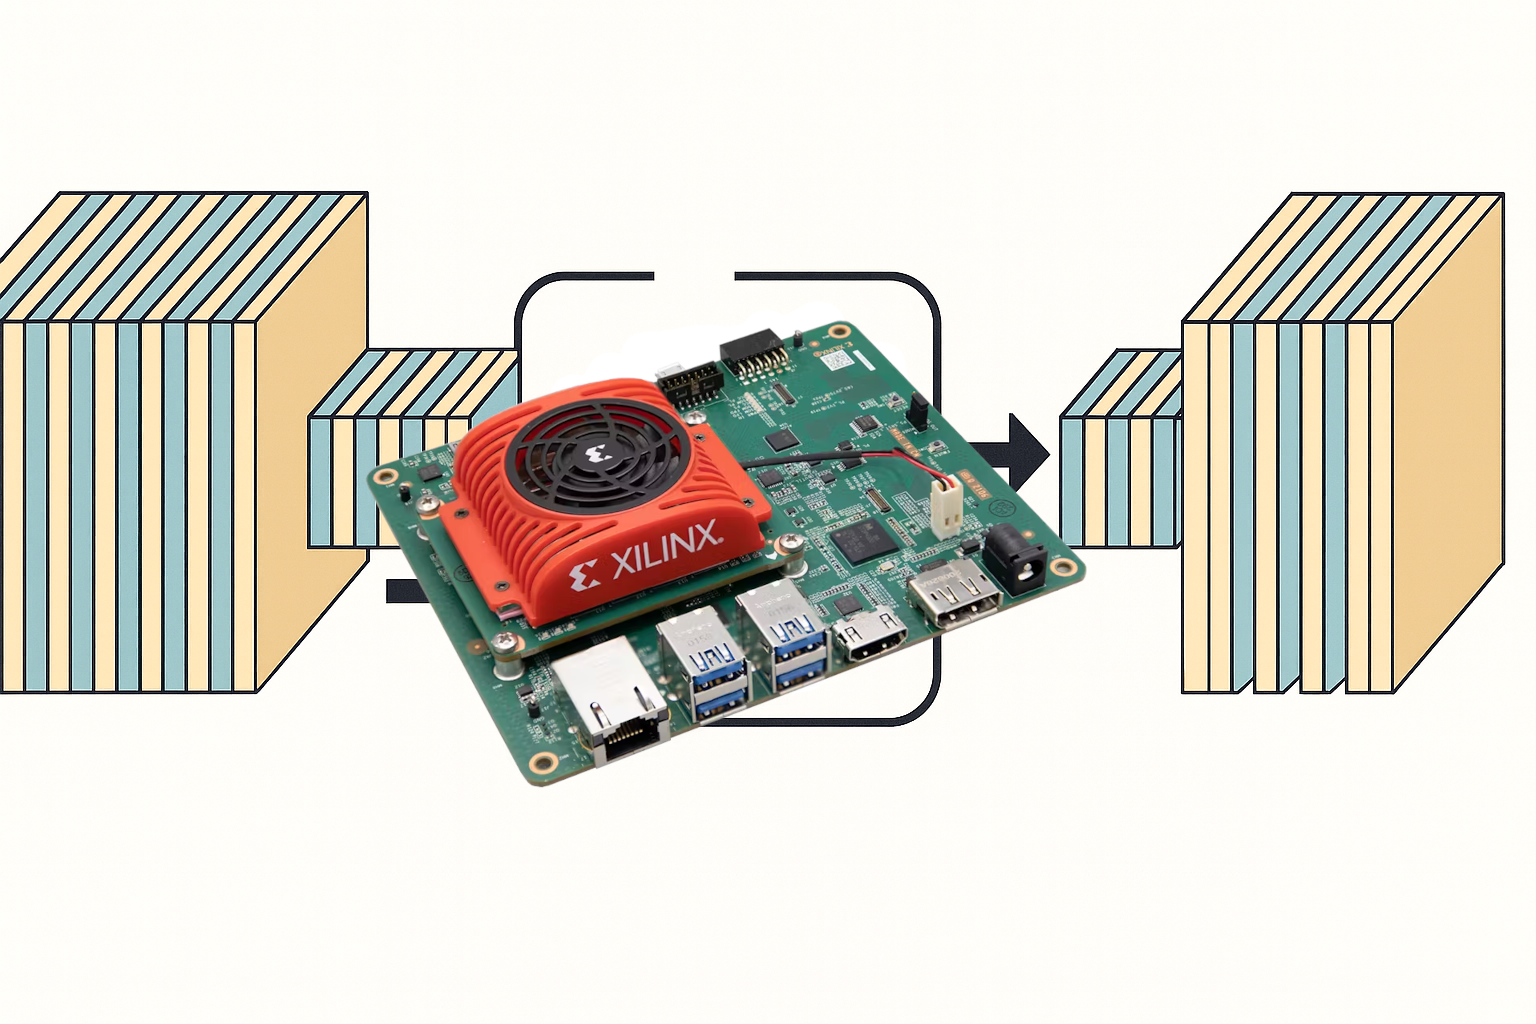
\includegraphics[width=0.15\textwidth]{../assets/title-logo.png}}

% Adjust title styling for readability
\settitle{
  \centering
  \vbox{
    \centering
    \@titlegraphic \\[\TP@titlegraphictotitledistance]
    \vspace*{1em}
    \color{titlefgcolor}
    {\bfseries \Huge \@title \par}
    \vspace*{1.5em}
    {\LARGE \textbf{Senior Design Project SDDEC25--01} \par}
    \vspace*{0.8em}
    {\Large Conner Ohnesorge, Tyler Schaefer, Aidan Perry, Joey Metzen \par}
    \vspace*{0.5em}
    {\Large Iowa State University \par}
    \vspace*{0.3em}
    {\large Department of Electrical and Computer Engineering}
  }
}

\begin{document}

\maketitle

% Two-column layout for better content organization
\begin{columns}
  \column{0.5}

  % LEFT COLUMN

  \block{Problem \& Approach}{
    % Introduction section for VisionAssist poster
% Problem statement and motivation

\textbf{The Problem:}

Wheelchair users face sudden medical episodes with no autonomous safety response.

\vspace{1em}

\begin{center}
\textit{[Visual: Storyboard showing wheelchair user experiencing medical distress]}
\end{center}

\vspace{1em}

\textbf{Our Solution:}

AI-powered eye tracking for proactive medical monitoring.

\vspace{1em}

\textbf{Key Features:}

\begin{itemize}
  \item Real-time pupil tracking (60 FPS)
  \item Privacy-preserving on-device processing
  \item Sub-100ms emergency response capability
  \item Designed for cerebral palsy \& epilepsy monitoring research
\end{itemize}

\vspace{1em}

\textbf{Scope:} This is a \textit{research prototype} exploring eye movement pattern analysis. Clinical validation with target populations is planned as future work.

  }

  \block{System Architecture}{
    % System Architecture section for VisionAssist poster
% Visual pipeline diagram

\textbf{End-to-End Processing Pipeline:}

\vspace{1em}

\begin{center}
% TODO: Create system block diagram showing:
% Camera → Preprocessing → U-Net Segmentation (DPU) → Feature Extraction → Output
% Include timing annotations (8.3ms per frame, 60 FPS total)
% Show pipelined scheduling visualization
\fbox{\parbox{0.9\linewidth}{
  \centering
  \vspace{2em}
  \textbf{[System Architecture Diagram]}\\[1em]
  Camera Input $\rightarrow$ Preprocessing $\rightarrow$ U-Net (DPU) $\rightarrow$ Feature Extraction $\rightarrow$ Eye Tracking Output\\[1em]
  \textit{8.3ms per frame | 60 FPS throughput | Pipelined DPU scheduling}
  \vspace{2em}
}}
\end{center}

\vspace{1em}

\textbf{Processing Steps:}

\begin{enumerate}
  \item Image capture \& preprocessing (gamma, CLAHE)
  \item U-Net segmentation on DPU accelerator
  \item Pupil detection \& blink classification
  \item Real-time feature tracking
\end{enumerate}

  }

  \block{Hardware \& AI Model}{
    % Methodology section for VisionAssist poster
% Technical approach and system architecture

\textbf{System Architecture:}

VisionAssist implements a sophisticated pipelined processing architecture optimized for real-time medical monitoring on resource-constrained embedded hardware.

\vspace{0.5em}

\textbf{Hardware Platform:}

\begin{itemize}
	\item \textbf{AMD Kria KV260:} Zynq UltraScale+ MPSoC development board
	\item Quad-core ARM Cortex-A53 processor (1.5 GHz)
	\item Deep Learning Processing Unit (DPU) for neural network acceleration
	\item 4GB DDR4 memory with four banks for parallel access
	\item Optimized for edge AI with low power consumption
\end{itemize}

\vspace{0.5em}

\textbf{AI Model: U-Net Semantic Segmentation}

\begin{center}
	\includegraphics[width=0.9\linewidth]{../assets/unet.png}
\end{center}

The U-Net architecture provides optimal balance for eye tracking:
\begin{itemize}
	\item Encoder-decoder structure with skip connections
	\item Preserves fine-grained spatial information for pupil detection
	\item Model compressed and quantized for DPU acceleration
	\item 98.8\% IoU accuracy maintained through optimization
\end{itemize}

\vspace{0.5em}

\textbf{Processing Pipeline:}

\begin{enumerate}
	\item \textbf{Image Capture:} Raw camera input acquisition from eye tracking camera
	\item \textbf{Preprocessing:} Image normalization, gamma correction (0.8 exponent), CLAHE contrast enhancement
	\item \textbf{Semantic Segmentation:} U-Net inference on DPU with pipelined processing
	\item \textbf{Feature Extraction:} Pupil identification, blink detection, position tracking
	\item \textbf{Medical Monitoring:} Real-time analysis for distress indicators
	\item \textbf{Safety Response:} Autonomous wheelchair repositioning when medical episode detected
\end{enumerate}

\vspace{0.5em}

\textbf{Key Technical Innovation:}

Our pipelined architecture achieves near 5x throughput improvement through efficient scheduling of the single DPU resource across multiple algorithms (semantic segmentation, blink detection, eye tracking) while maintaining accuracy. The system implements sequential DPU scheduling with fair resource allocation, ensuring all algorithms meet their periodic data collection requirements without starvation.

\vspace{0.5em}

\textbf{Critical Requirements Met:}

\begin{itemize}
	\item \textbf{Latency:} <100ms for medical emergency detection and response
	\item \textbf{Accuracy:} 98.8\% IoU for semantic segmentation (target: 99.8\%)
	\item \textbf{Throughput:} 60 FPS (4 frames in <33.2ms)
	\item \textbf{Privacy:} All processing on-device, no external data transmission
\end{itemize}

  }

  \column{0.5}

  % RIGHT COLUMN

  \block{Performance \& Validation}{
    % Results section for VisionAssist poster
% Performance metrics and achievements

\textbf{Achieved Performance:}

\begin{center}
\begin{tabular}{lr}
\toprule
\textbf{Metric} & \textbf{Result} \\
\midrule
Throughput & 60 FPS \\
Latency (4 frames) & <33.2 ms \\
Segmentation Accuracy (IoU) & 98.8\% \\
Continuous Operation & 24+ hours \\
\bottomrule
\end{tabular}
\end{center}

\vspace{1em}

\textbf{What This Means:}

\begin{itemize}
  \item \textbf{60 FPS:} Enables smooth, responsive eye movement tracking
  \item \textbf{98.8\% IoU:} Accurate pupil detection across lighting conditions
  \item \textbf{24+ hours:} Reliable for all-day wheelchair use
  \item \textbf{On-device:} No network dependency, preserves privacy
\end{itemize}

\vspace{1em}

\textbf{System Validation:}

\begin{itemize}
  \item \textbf{Lighting robustness:} >98\% accuracy in varied conditions
  \item \textbf{Scheduling fairness:} Zero missed deadlines under load
  \item \textbf{IEEE compliance:} Testing per IEEE 3129--2023 \& IEEE 2802--2022
\end{itemize}

\vspace{1em}

\textbf{Limitations:}

This is a \textit{proof-of-concept}. Clinical validation with wheelchair users is required before deployment. Current focus: engineering performance, not medical efficacy.

  }

  \block{Impact \& Next Steps}{
    % Conclusion section for VisionAssist poster
% Impact, achievements, and future work

\textbf{Key Achievement:}

\textbf{5× throughput improvement} through pipelined DPU scheduling—proves intelligent resource allocation outperforms hardware upgrades.

\vspace{1em}

\textbf{Safety \& Ethics:}

\begin{itemize}
  \item \textbf{Fail-safe design:} System defaults to safe state on failure
  \item \textbf{User autonomy:} Monitoring does not override user control
  \item \textbf{Privacy-first:} Zero external data transmission
  \item \textbf{Accessibility:} Designed for diverse user needs
\end{itemize}

\vspace{1em}

\textbf{Next Steps:}

\begin{itemize}
  \item \textbf{IRB-approved user studies} with wheelchair users
  \item \textbf{Medical device certification} pathway
  \item \textbf{Integration with caregiver alert systems}
  \item \textbf{Refinement:} Target 99.8\% IoU accuracy
\end{itemize}

\vspace{1em}

\textbf{Impact:}

This project demonstrates that \textit{edge AI can enable privacy-preserving assistive technologies} without requiring cloud infrastructure or expensive hardware—making advanced monitoring more accessible to individuals with disabilities.

  }

\end{columns}

% Bottom section spanning full width
\block{Acknowledgments}{
  % Acknowledgments section for VisionAssist poster
% Credits and institutional support

\textbf{Acknowledgments:}

\vspace{0.5em}

We gratefully acknowledge the support and contributions that made
this project possible:

\vspace{0.5em}

\textbf{Institutional Support:}
\begin{itemize}
  \item Iowa State University Department of Electrical and Computer Engineering
  \item Senior Design Program (SDDEC 2025)
  \item Computer Engineering faculty and staff
\end{itemize}

\vspace{0.5em}

\textbf{Project Team:}
\begin{itemize}
  \item Conner Ohnesorge
  \item Tyler Schaefer
  \item Aidan Perry
  \item Joey Metzen
\end{itemize}

\vspace{0.5em}

\textbf{Technical Resources:}
\begin{itemize}
  \item AMD Xilinx for Kria KV260 development platform and Vitis AI tools
  \item Previous Iowa State project teams for foundational system architecture
  \item Open-source community (PyTorch, ONNX, OpenEDS dataset)
  \item Precomputed training dataset: \texttt{Conner/openeds-precomputed} on HuggingFace Hub
\end{itemize}

\vspace{0.5em}

\textbf{Project Client:} JR Spidell
\begin{itemize}
  \item Domain expertise in assistive wheelchair technology
  \item Requirements specification and medical use case validation
\end{itemize}

\vspace{0.5em}

\textbf{Faculty Advisor:} Dr.~Namrata Vaswani
\begin{itemize}
  \item Technical guidance and project oversight
  \item Department of Electrical and Computer Engineering, Iowa State University
\end{itemize}

\vspace{0.5em}

\textbf{Standards and Compliance:}
\begin{itemize}
  \item IEEE for standards guidance (IEEE 3129--2023, IEEE 2802--2022)
\end{itemize}

\vspace{1em}

\textit{This project demonstrates interdisciplinary collaboration in
  assistive technology, combining artificial intelligence, embedded
  systems engineering, and medical device design to enhance
independence and safety for individuals with disabilities.}

}

% Bibliography section at bottom
\block{References}{
  \printbibliography[heading=none]
}

\end{document}
